1996年,第一个SIMD(根据Flynn的分类法,Single Instruction, Multiple Data)指令集是在x86架构之上的MMX。从那以后,许多SIMD指令集扩展既遵循Intel架构,也在行业中都广泛的应用。CPU核心通过执行指令来完成它的工作,核心知道如何执行特定的指令是由它实现的指令集(如x86, x86\_64, AltiVec, NEON)和指令集扩展(如SSE, AVX, AVX-512)定义的。指令集扩展添加的许多操作都集中在SIMD指令上。\par

通过使用比处理的数据基本单元更大的寄存器和硬件,SIMD指令允许在单个核上同时执行多个计算。使用512位寄存器,这样可以用一条机器指令执行8个64位计算。\par

\hspace*{\fill} \par %插入空行
图16-2 在CPU硬件线程中执行SIMD
\begin{center}
	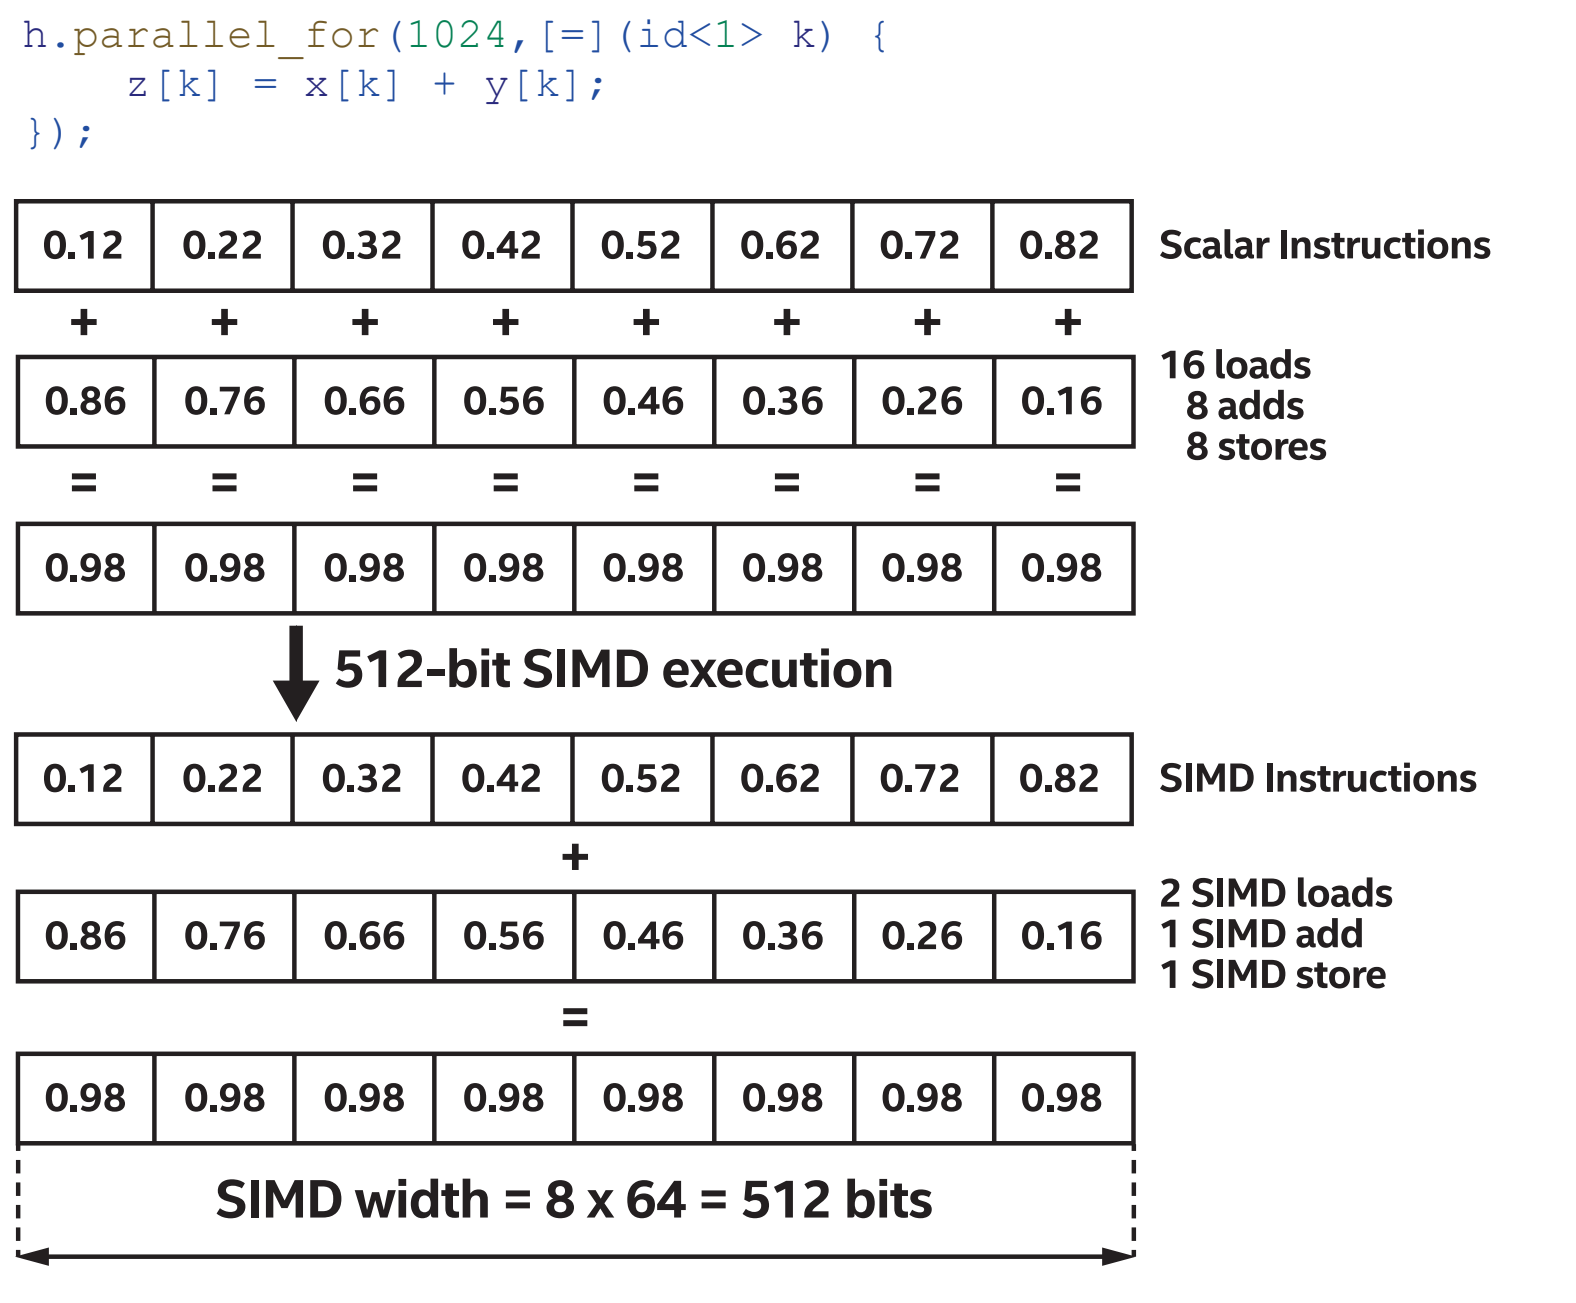
\includegraphics[width=1.0\textwidth]{content/chapter-16/images/3}
\end{center}

图16-2的这个例子可以带来8倍的加速。实际中,可能在达不到8倍,这是瓶颈可能不完全在计算上,也有部分在内存吞吐量上。通常,使用SIMD的性能优势取决于特定的场景。在一些情况下,甚至比更简单的非SIMD等效代码的性能更差。现代处理器上,如果知道何时以及如何应用(或让编译器应用)SIMD,就可以获得可观的收益。与所有性能优化一样,开发者应该在将目标机器投入生产之前,测试其性能收益。本章接下来的章节中有更多关于预期性能提高的细节。\par

具有SIMD单元的cc-NUMA CPU体系结构,构成了多核处理器的基础,可以以五种不同的方式利用指令级并行,如图16-3所示。\par

\hspace*{\fill} \par %插入空行
图16-3 五种并行执行指令的方法
\begin{center}
	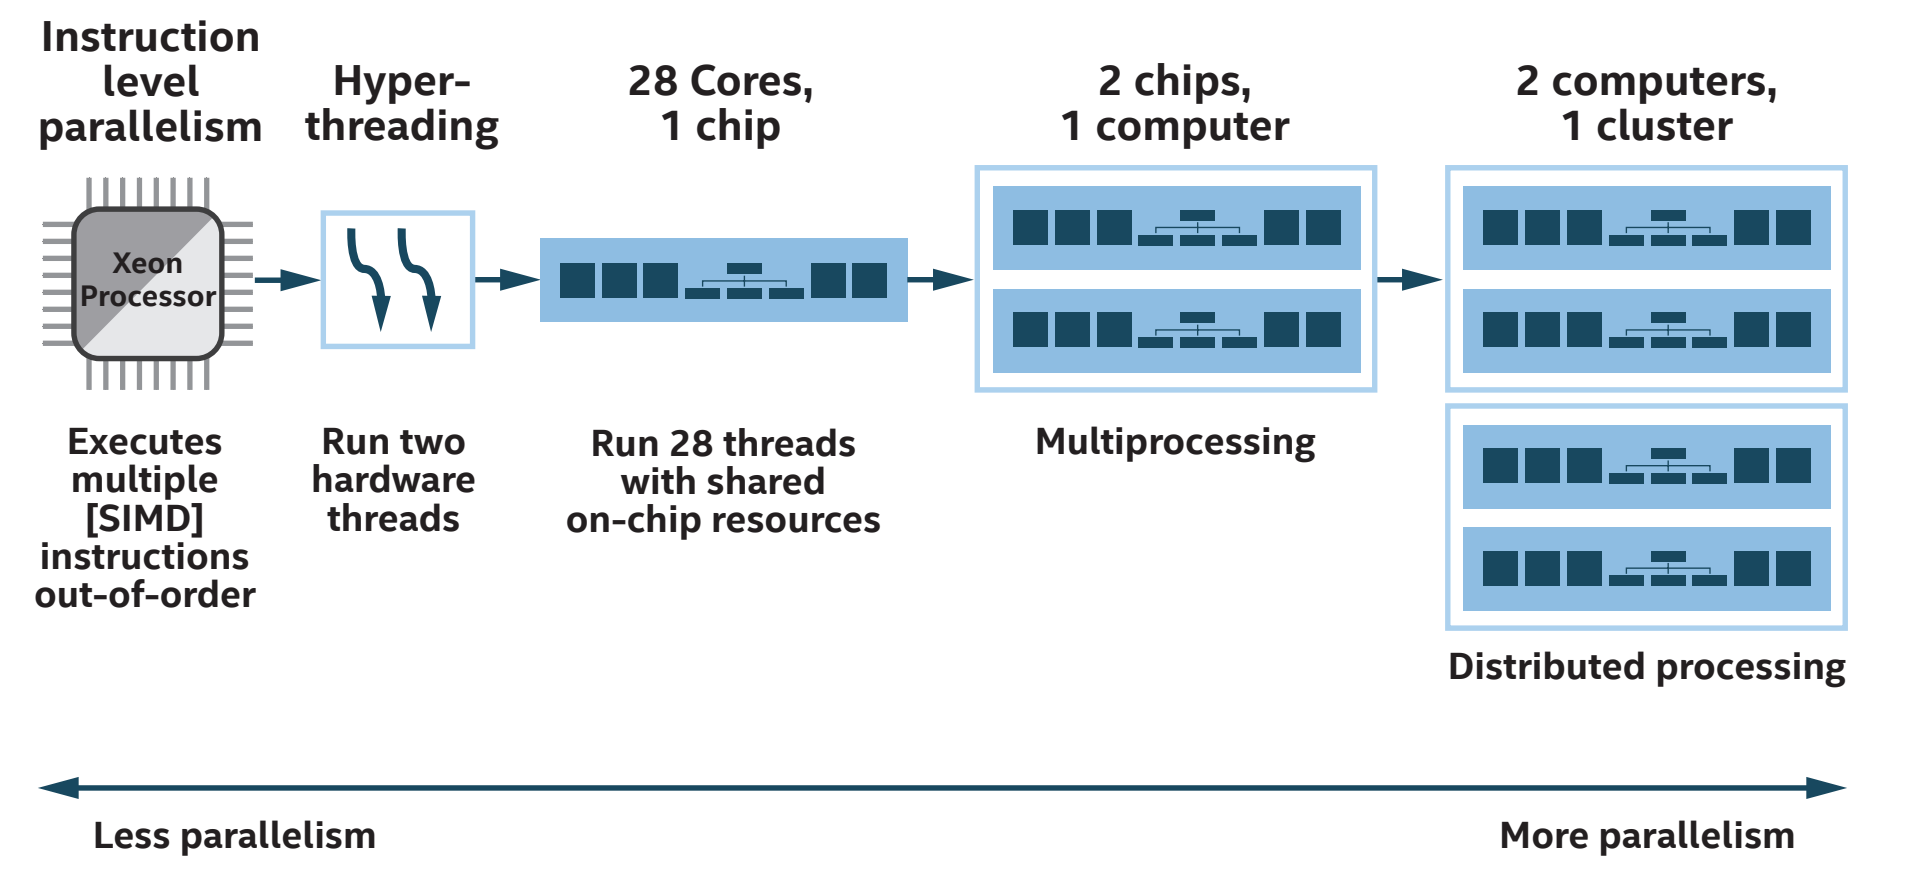
\includegraphics[width=1.0\textwidth]{content/chapter-16/images/4}
\end{center}

图16-3中,指令级并行可以通过标量指令的无序执行实现,也可以通过单个线程中的SIMD (Single Instruction, Multiple Data)数据并行实现。线程级并行可以通过在同一个核或不同规模的多个核上执行多个线程来实现。更具体地说,线程级并行性可以通过以下方式实现:\par

\begin{itemize}
	\item 现代CPU体系结构允许一个核芯同时执行两个或多个线程的指令。
	\item 每个处理器中包含两个或多个多核架构。操作系统将每个执行核心视为具有所有相关执行资源的独立处理器。
	\item 处理器(芯片)级的多处理,可以通过独立的线程来完成。因此,处理器可以在应用中运行线程,在操作系统中运行另一个线程,或者可以在单个应用程序中运行并行线程。
	\item 分布式处理,可以通过在计算机集群上执行由多个线程组成的进程来完成,这些进程通常通过消息传递框架进行通信。
\end{itemize}

为了充分利用多核处理器资源,软件必须将工作负载分布到多个核的方式编写。这种方法利用了线程级并行性或简单的线程化。\par

随着多处理器计算机和具有超线程(HT)技术的多核处理器越来越多,将并行处理技术作为提高性能的标准实践是非常重要的。本章后面的部分将介绍DPC++中的编码方法和性能调优技术,这些技术允许在多核CPU上实现最高性能。\par

与其他并行处理硬件(例如GPU)一样,给CPU足够大的数据元素集来处理很重要。为了说明如何利用多级并行处理大量数据的重要性,请考虑一个简单的C++ STREAM Triad程序,如图16-4所示。\par

\begin{tcolorbox}[colback=blue!5!white,colframe=blue!75!black, title=关于STREAM Triad工作负载的解释]
STREAM Triad工作负载(www.cs.virginia.edu/stream)是一个基准工作负载,CPU供应商使用它来演示高度调优的性能。使用STREAM Triad内核来演示并行内核的代码生成,以及通过本章描述的技术来实现显著提高性能的计划方式。STREAM Triad是一个相对简单的工作负载,但足以显示许多优化。
\end{tcolorbox}

\begin{tcolorbox}[colback=blue!5!white,colframe=blue!75!black, title=使用供应商提供的库!]
当供应商提供函数库实现时,使用它而不是将函数重新实现为并行内核!
\end{tcolorbox}

\hspace*{\fill} \par %插入空行
图16-4 STREAM Triad C++循环
\begin{lstlisting}[caption={}]
// C++ STREAM Triad workload
// __restrict is used to denote no memory aliasing among arguments 
template <typename T>
double triad(T* __restrict VA, T* __restrict VB, 
			 T* __restrict VC, size_t array_size, const T scalar) {
	double ts = timer_start()
	for (size_t id = 0; id < array_size; id++) {
		VC[id] = VA[id] + scalar * VB[id];
	}
	double te = timer_end();
	return (te – ts); 
}
\end{lstlisting}

STREAM Triad循环可以在CPU上简单地执行,使用单个CPU进行串行执行。好的C++编译器会将执行循环向量化,为具有SIMD硬件的CPU生成SIMD代码,以便利用指令级的SIMD并行性。例如,对于支持AVX-512的Intel Xeon处理器,Intel C++编译器生成SIMD代码,如图16-5所示。编译器对代码的转换减少了执行时的循环迭代次数,这是通过在运行时每个循环迭代执行更多的工作(SIMD宽度和展开的迭代)!\par

\hspace*{\fill} \par %插入空行
图16-5 TREAM Triad C++循环的AVX-512代码
\begin{lstlisting}[caption={}]
// STREAM Triad: SIMD code generated by the compiler, where zmm0, zmm1 
// and zmm2 are SIMD vector registers. The vectorized loop is unrolled by 4
// to leverage the out-of-execution of instructions from Xeon CPU and to
// hide memory load and store latency 

# %bb.0: # %entry
vbroadcastsd %xmm0, %zmm0 # broadcast “scalar” to SIMD reg zmm0
movq $-32, %rax
.p2align 4, 0x90
.LBB0_1: # %loop.19
# =>This Loop Header: Depth=1
vmovupd 256(%rdx,%rax,8), %zmm1 # load 8 elements from memory to zmm1 
vfmadd213pd 256(%rsi,%rax,8), %zmm0, %zmm1 # zmm1=(zmm0*zmm1)+mem
# perform SIMD FMA for 8 data elements 
# VC[id:8] = scalar*VB[id:8]+VA[id:8] 
vmovupd %zmm1, 256(%rdi,%rax,8) # store 8-element result to mem from zmm1 
# This SIMD loop body is unrolled by 4
vmovupd 320(%rdx,%rax,8), %zmm1
vfmadd213pd 320(%rsi,%rax,8), %zmm0, %zmm1 # zmm1=(zmm0*zmm1)+mem
vmovupd %zmm1, 320(%rdi,%rax,8)
vmovupd 384(%rdx,%rax,8), %zmm1
vfmadd213pd 384(%rsi,%rax,8), %zmm0, %zmm1 # zmm1=(zmm0*zmm1)+mem
vmovupd %zmm1, 384(%rdi,%rax,8)
vmovupd 448(%rdx,%rax,8), %zmm1
vfmadd213pd 448(%rsi,%rax,8), %zmm0, %zmm1 # zmm1=(zmm0*zmm1)+mem
vmovupd %zmm1, 448(%rdi,%rax,8)
addq $32, %rax
cmpq $134217696, %rax # imm = 0x7FFFFE0
jb .LBB0_1
\end{lstlisting}

如图16-5所示,编译器能以两种方式利用指令级并行性。首先是通过SIMD指令的使用,利用指令级数据并行性,其中一条指令可以同时并行处理8个双精度数据元素(每个指令)。其次,基于硬件多路指令调度,编译器循环展开来获得(指令之间没有依赖关系)乱序执行是效果。\par

如果尝试在CPU上执行这个函数,可能会运行得很好——没有利用CPU的任何多核或线程能力,对于小数组来说已经足够好了。但是,当试图在CPU上使用大数组来执行这个函数,那性能很可能会很差,因为单个线程只使用一个CPU核,当这个核的内存带宽饱和时就会出现性能瓶颈。\par

























































